\chapter{Ψηφιακό βίντεο και τεχνικές συμπίεσης}
\label{chapter:chap2}


\section{Εισαγωγή}
\label{section:sect21}
\indent
Σε αυτό το κεφάλαιο γίνεται μία εισαγωγή στους τρόπους που οι κωδικοποιητές βίντεο διαχειρίζονται τα δεδομένα και τους τρόπους που χρησιμοποιούν για να τα συμπιέσουν. Επίσης εδώ θα μας γίνει ξεκάθαρο γιατί το βήμα της κβαντοποίησης (εισαγωγή θορύβου) είναι αναγκαία για να έχουμε τόσο μεγάλους λόγους συμπίεσης

\section{Συστατικά στοιχεία του βίντεο}
\label{section:sect22}

\indent Το ψηφιακό βίντεο αποτελείται από μία σειρά καρέ που αναπαράγονται με σταθερό ρυθμό (συνήθως 25Hz η 30Hz). Το κάθε καρέ απεικονίζεται σε ένα χώρο χρωμάτων που ονομάζεται YUV, οπού το Y είναι η φωτεινότητα και το U,V το χρώμα. Η κάθε συνιστώσα στο ανθρώπινο μάτι φαίνεται στο Σχήμα~\ref{fig:yuv}.

\indent Σε κάθε σημείο του βίντεο(pixel) αντιστοιχίζεται μια τέτοια τιμή YUV. Υπάρχουν διάφοροι τρόποι που γίνεται αυτή η αντιστοίχηση με κυριότερες αυτές του YUV420 και YUV444. Η πρώτη μας λέει πως κάθε για κάθε τέσσερα pixel υπάρχουν τέσσερις τιμές Y μία τιμή U και μια τιμή V ενώ η δεύτερη πως για κάθε τέσσερα pixel υπάρχουν τέσσερις τιμές για την κάθε συνιστώσα π.χ για ένα καρέ ανάλυσης 720*480 τύπου YUV420 έχουμε \(720*480=345600\) στοιχεία Υ, \(720*480/4\) στοιχεία U και \(720*480/4 \) στοιχεία V αρά σύνολο 518400.Ο τρόπος αποθήκευσης του βίντεο γίνετε πάντα ανά καρέ και υπάρχουν δύο τρόποι, ο packed και ο planar. Στον πρώτο το YUV για κάθε pixel αποθηκεύεται με την σειρά ενώ στον δεύτερο και επικρατέστερο αποθηκεύεται πρώτα όλο το Y και μετά ακολουθούν τα U,V.

\indent Κάθε pixel έχει και ένα βάθος (bitdepth), δηλαδή ποιο είναι το εύρος τιμών που παίρνει. Οι σύγχρονοι κωδικοποιητές υποστηρίζουν 8-14bits έτσι συνεχίζοντας το παράδειγμα μας από την προηγούμενη παράγραφο και έχοντας συνολικά 518400 στοιχεία για ένα καρέ και υποθέτοντας ότι το bitdepth=8 τότε συνολικά χρειαζόμαστε 518400*8bits $\approx$ 0.5MB. Το πιο κοινό bitdepth που χρησιμοποιείται από τους σημερινούς κωδικοποιητές είναι αυτό τον 8bits.

\begin{figure}[p]
    
    \centering
        
\includegraphics[totalheight=0.9\textheight,width=0.5\textwidth]{chapter2/yuv.jpg}
    \caption{Στην πρώτη εικόνα φαίνεται ένα καρέ με όλες τις συνιστώσες ενώ παρακάτω ξεχωριστά το YUV για το ίδιο καρέ.}
    \label{fig:yuv}
\end{figure}

\newpage
\section{Οργάνωση των pixels από τους κωδικοποιητές}
\label{section:sect23}

\indent Η πλειοψηφία των σημερινών κωδικοποιητών ομαδοποιούν τα pixels. Η πιο συνηθισμένη ομαδοποίηση είναι αυτή του macroblock, οπού το κάθε καρέ διαιρείται σε μικρά πλακίδια σταθερής διάστασης NxN pixels οπού συνήθως N$=$16. Έτσι το καρέ του παραδείγματος μας αποτελείται από 518400/(16*16) $=$ 2025 macroblocks. Το κάθε macroblock μπορεί να σπάσει σε blocks και το κάθε block σε subblocks όπως φαίνεται στο Σχήμα~\ref{fig:mbpart}.

\begin{figure}[h!]
  
  \centering
    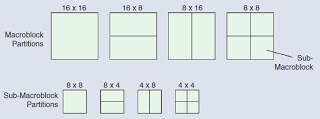
\includegraphics[width=0.5\textwidth]{chapter2/mbpart.jpg}
  \caption{Διαμερισμός του macroblock στον H.264.}
  \label{fig:mbpart}
\end{figure}

\indent Μέτα τον χωρισμό σε macroblocks οι κωδικοποιητές ομαδοποιούν τα καρέ σε Intra και Inter οπού τα τελευταία χωρίζονται σε P και Β. Όλες οι παραπάνω κατηγοριοποιήσεις έχουν να κάνουν με τον μηχανισμό του Motion Estimation οπού ο encoder δημιουργεί διαφορές pixels (residuals). Τα residuals έχουν μικρότερη ενεργεία οπότε είναι οι διάφοροι μετασχηματισμοί που εφαρμόζονται αργότερα στην αλυσίδα μας δίνουν μικρότερη ενεργεία και επιπλέον περισσότερα μηδενικά.

\begin{itemize}
  \item Intra η αλλιώς I είναι τα καρέ που χρησιμοποιούν πληροφορία μόνο από το τρέχων καρέ για να βγάλουν τα residuals. Αυτό γίνετε απλά παίρνοντας τις τιμές των γειτονικών block και εφαρμόζοντας μια πράξη π.χ μέσος όρος οπού το αποτέλεσμα αυτής αφαιρείται από τις τιμές των pixel του τρέχων block. Υπάρχουν διάφορες πράξεις που μπορούν να γίνουν όπως φαίνεται και στο Σχήμα~\ref{fig:intrapred} και δοκιμάζονται κάθε φόρα όλες μέχρι να καταλήξουμε στην καλύτερη. Η απόδοση της συμπίεσης είναι η χειρότερη σε αυτήν την κατηγορία αλλά χωρίς αυτά το βίντεο δε θα μπορούσε να ξεκινήσει γιατί δεν θα είχαμε όλη την πληροφορία.

  \item P καρέ είναι αυτά τα οποία ψάχνουν το καλύτερο block για να κάνουν διαφορές από κάποιο αριθμό προηγούμενων καρέ όπως φαίνεται στο Σχήμα~\ref{fig:gop}

  \item Β καρέ είναι αυτά τα οποία ψάχνουν το καλύτερο block για να κάνουν διαφορές από κάποιο αριθμό προηγούμενων αλλά και επόμενων καρέ όπως φαίνεται στο Σχήμα~\ref{fig:gop}. Αυτά έχουν την καλύτερη απόδοση συμπίεσης αλλά η πολυπλοκότητα αποκωδικοποίησης είναι η μεγαλύτερη.
\end{itemize}

\indent Ένα επιπλέον στοιχείο των encoder είναι το group of pictures (GOP) οπού αυτό χαρακτηρίζει την σειρά με την οποία τα είδη των καρέ τοποθετούνται. Το GOP ξεκινάει από ένα I-frame συνεχίζει με P,B και περιοδικά έρχεται ένα Ι. Το GOP εξαρτάται από την εφαρμογή και μπορεί να διαφέρει κατά πολύ. Ένα τυπικό φαίνεται στο Σχήμα~\ref{fig:gop}

\begin{figure}[h!]
  
  \centering
    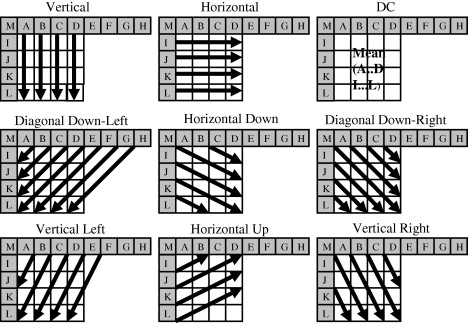
\includegraphics[width=0.5\textwidth]{chapter2/intrapred.jpg}
  \caption{Τρόποι που χρησιμοποιούνται στον Η.264 για Intra prediction}
    \label{fig:intrapred}
\end{figure}

\begin{figure}[h!]
  
  \centering
    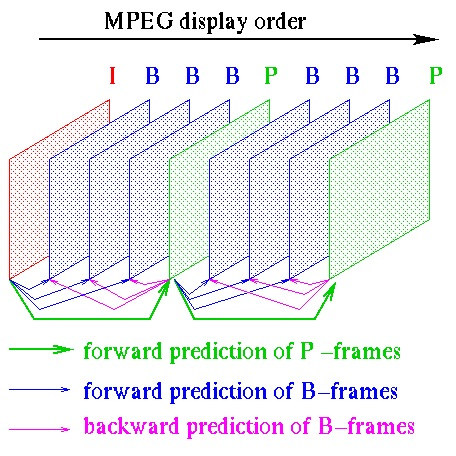
\includegraphics[width=0.5\textwidth]{chapter2/gop.jpg}
  \caption{Inter prediction στον mpeg και απεικόνιση ενός ενδεικτικοί GOP }
  \label{fig:gop}
\end{figure}

\newpage
\section{Μετασχηματισμός}
\label{section:sect24}

\indent Αφού ο encoder έχει κατασκευάσει τα residuals για το macroblock τότε το επόμενο βήμα είναι ένας μετασχηματισμός οπού συνήθως είναι ο DCT. Αυτό συμβαίνει γιατί ο μετασχηματισμός μας επιστρέφει πολλά 0 αν το σήμα μας είναι χαμηλής ενέργειας, όπως συμβαίνει με τα residuals. Έτσι χρησιμοποιώντας κάποιο ειδικό σύμβολο μπορούν να απεικονιστούν πολλά μηδενικά του μετασχηματισμού και να μειώσουμε το data rate μας όπως φαίνεται στο Σχήμα~\ref{fig:rle}. Η σάρωση του macroblock δεν γίνετε γραμμικά αλλά με την μέθοδο του zigzag όπως στο Σχήμα~\ref{fig:zigzag} γιατί έτσι έχει παρατηρηθεί πως έχουμε παραπάνω μηδενικά στην σειρά.

\begin{figure}[h!]
  
  \centering
    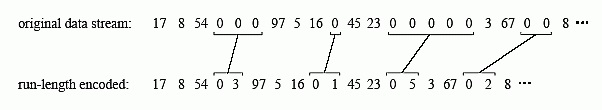
\includegraphics[totalheight=0.2\textheight,width=0.8\textwidth]{chapter2/rle.jpg}
  \caption{Παράδειγμα ένωσης μηδενικών}
  \label{fig:rle}
\end{figure}

\begin{figure}[h!]
  
  \centering
  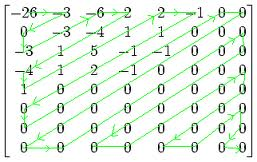
\includegraphics[width=0.5\textwidth]{chapter2/zigzag.jpg}
  \caption{Σάρωση ZigZag}
  \label{fig:zigzag}
\end{figure}

\newpage
\section{Κβαντοποίηση}
\label{section:sect25}

\indent Η κβαντοποίηση είναι το σημείο που σε κάθε encoder εισάγεται ο θόρυβος, θα μπορούσε να θεωρηθεί και ο DCT,iDCT λόγο ακρίβειας αλλά εκεί το σφάλμα είναι παρά πολύ μικρό. Μετά τον μετασχηματισμό τα residuals έχουν αντικατασταθεί με συντελεστές οι οποίοι είναι πραγματικοί αριθμό. Η τακτική που εφαρμόζεται είναι να γίνει ακέραια διαίρεση ο συντελεστής της κάθε συχνότητας με έναν σταθερό αριθμό διαφορετικό για κάθε συχνότητα Σχήμα~\ref{fig:quanttable}. Επομένως για τον δεδομένο πίνακα κβαντοποίησης με τους συντελεστές του Σχήματος ~\ref{fig:coeff} έχουμε τα αποτελέσματα του Σχήματος ~\ref{fig:results} έτοιμα προς κωδικοποίηση με κάποιον entropy encoder και εγγραφή.

\begin{figure}[h!]
\centering
  
  
    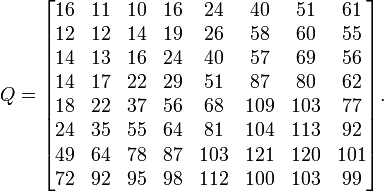
\includegraphics[width=0.5\textwidth]{chapter2/quanttable.png}
  \caption{Παράδειγμα πίνακα κβαντοποίησης για μετασχηματισμό 8x8}
  \label{fig:quanttable}
\end{figure}

\begin{figure}[h!]
    \centering 
    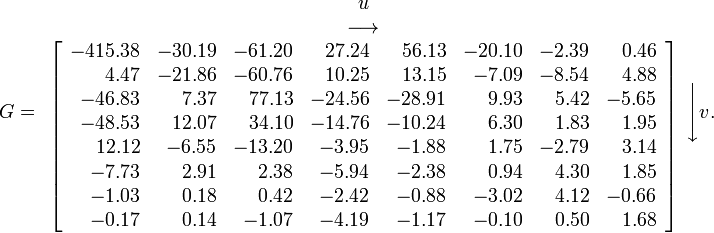
\includegraphics[width=0.5\textwidth]{chapter2/coeff.png}  
    \caption{Παράδειγμα συντελεστών DCT 8x8}
    \label{fig:coeff}
\end{figure}

\begin{figure}[h!]
    \centering    
    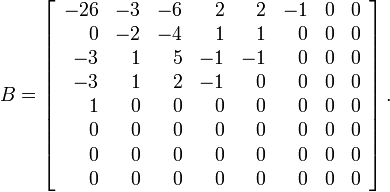
\includegraphics[width=0.5\textwidth]{chapter2/results.png}
    \caption{Παράδειγμα συντελεστών DCT 8x8}
    \label{fig:results}
\end{figure}

\indent Παρακάτω βλέπουμε την δομή του H.264 οπού επίτηδες έχω παραλείψει να αναφερθώ σε κάποια κομμάτια τους αφού δεν κρίνονται αναγκαία για την κατανόηση αυτής της διπλωματικής.

\begin{figure}[h]
    \centering  
    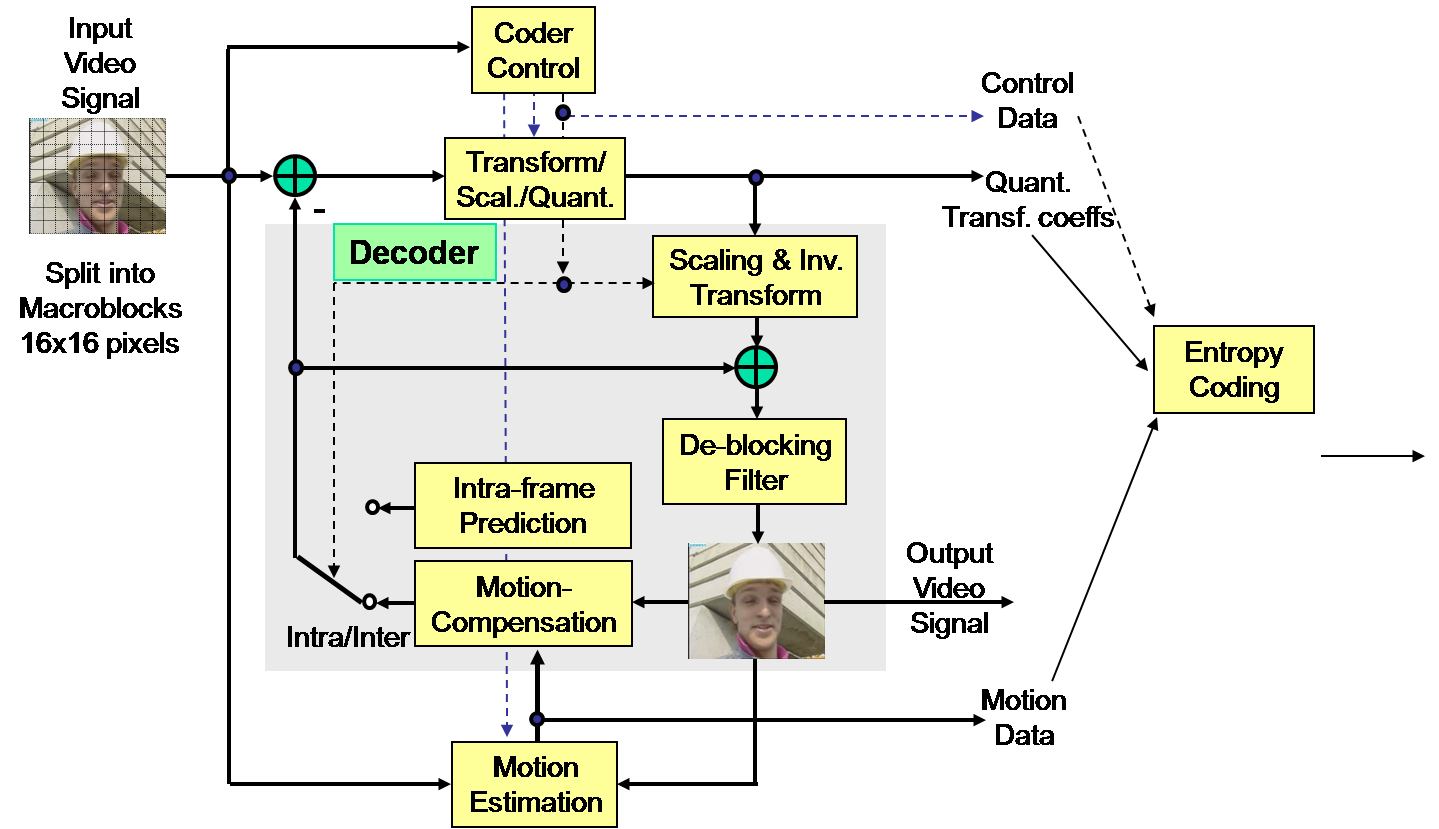
\includegraphics[width=0.5\textwidth]{chapter2/h264.png}
    \caption{H.264 structure}
    \label{fig:h264}
\end{figure}

\newpage

\section{Αποκωδικοποίηση βίντεο}
\label{section:sect26}

\indent Για την αποκωδικοποίηση κάνουμε όλα τα βήματα προς τα πίσω.

\begin{itemize}
  \item Μετά την entropy decoding πολλαπλασιάζουμε τα νούμερα με τα στοιχεία του πίνακα κβαντοποίησης. Έτσι παίρνουμε τους DCT συντελεστές αλλά λανθασμένους λόγο της ακέραιας διαίρεσης.
  \item Έπειτα κάνουμε iDCT και παίρνουμε τα residuals.
  \item Τελευταίο βήμα είναι να κάνουμε το Motion Decomposition βρίσκοντας τα δύο block που χρησιμοποιήθηκαν για να παραχθούν τα residuals και τα προσθέτουμε για να πάρουμε τα ανακατασκευασμένα pixels.
\end{itemize}